% Part III-A, results of the GRPO runs (included by main_en.tex).
% DRAFT, written with 5 of the 6 runs (hidden seed 2 missing); every claim is to be checked against all six.

\section{Training against the visible tests}\label{sec:res-grpo}

Each reward trained the policy for 100 steps (16 problems with 8 episodes each, learning rate $10^{-5}$ as in Part II)
with \NUM{cgseeds_vis} seeds. Table~\ref{tab:code-grpo} gives the final policies on the three evaluation sets,
Table~\ref{tab:code-paired} the paired differences between rewards, and Figure~\ref{fig:code-curves} the training
curves. The 95\% intervals resample problems; they do not include the variation between seeds, so we also give each
seed's value where the seeds disagree.

\paragraph{Training on the visible tests made the code more correct.} At step 0 the base policy passes every test on
\NUM{cgszmean_kod_allpass}\% of the KodCode validation problems, \NUM{cgszmean_mbpp_allpass}\% of MBPP+ and
\NUM{cgszmean_he_allpass}\% of HumanEval+. After 100 steps with the \texttt{vis} reward it passes every test on
\NUM{cgall_vis_kod}\%, \NUM{cgall_vis_mbpp}\% and \NUM{cgall_vis_he}\%, and it needs fewer repairs: it solves
\NUM{cgfirst_vis_kod}\% of the KodCode validation problems at the first attempt, against
\NUM{cgszmean_kod_firstattemptallpass}\% at step 0. MBPP+ and HumanEval+ were never trained on.

\paragraph{The gap between visible and held-out tests shrank on two sets, not on MBPP+.} Of the base policy's
visible-test passes on KodCode validation, \NUM{cgszmean_kod_hackamongvispass}\% fail a held-out test; after training
\NUM{cghackv_vis_kod}\% do. On HumanEval+ the share falls from \NUM{cgszmean_he_hackamongvispass}\% to
\NUM{cghackv_vis_he}\%. On MBPP+ it barely moves, from \NUM{cgszmean_mbpp_hackamongvispass}\% to
\NUM{cghackv_vis_mbpp}\%: the policy passes many more of MBPP+'s visible tests (\NUM{cgszmean_mbpp_vispass}\% of the
problems at step 0, \NUM{cgvis_vis_mbpp}\% after training), and the problems where the visible tests pass but a held-out
test fails grow from \NUM{cgszmean_mbpp_hack}\% to \NUM{cghack_vis_mbpp}\% of all problems. Training did not make the
policy more fitted to the visible tests than the base policy was, but on MBPP+ it did not make it less fitted either.

\begin{table}[t]
\centering\small
\begin{tabular}{@{}lcccccccccc@{}}
\toprule
 & & \multicolumn{3}{c}{KodCode val} & \multicolumn{3}{c}{MBPP+} & \multicolumn{3}{c}{HumanEval+} \\ \cmidrule(lr){3-5}\cmidrule(lr){6-8}\cmidrule(lr){9-11}
condition & seeds & vis & all & hack & vis & all & hack & vis & all & hack \\ \midrule
\texttt{vis} & 2 & 97.1 & 86.6 & 10.6 & 84.7 & 69.3 & 15.4 & 88.5 & 76.4 & 12.1 \\
\texttt{vis\_kev} & 2 & 96.6 & 86.6 & 10.1 & 85.2 & 72.3 & 12.9 & 87.9 & 76.7 & 11.2 \\
\texttt{hidden} & 2 & 96.3 & 87.2 & 9.1 & 82.0 & 68.8 & 13.3 & 88.2 & 77.0 & 11.2 \\
\bottomrule
\end{tabular}

\caption{Final policies (greedy, up to three attempts): visible tests pass (\emph{vis}), every test passes
(\emph{all}), and visible tests pass but a held-out test fails (\emph{hack}), in percent of problems; seed means.}
\label{tab:code-grpo}
\end{table}

\paragraph{The oracle reward removes some wrong passes, not more problems solved.} \texttt{hidden} pays only for code
that passes every test, so it never pays for a wrong program. Its final policy solves as many problems as
\texttt{vis}'s: all-pass differs by \NUM{cgdall_hidden_kod} \ci{\NUM{cgdalllo_hidden_kod}}{\NUM{cgdallhi_hidden_kod}}
points on KodCode validation, \NUM{cgdall_hidden_mbpp} \ci{\NUM{cgdalllo_hidden_mbpp}}{\NUM{cgdallhi_hidden_mbpp}} on
MBPP+ and \NUM{cgdall_hidden_he} \ci{\NUM{cgdalllo_hidden_he}}{\NUM{cgdallhi_hidden_he}} on HumanEval+
(Table~\ref{tab:code-paired}). It passes the visible tests less often (\NUM{cgvis_hidden_mbpp}\% against
\NUM{cgvis_vis_mbpp}\% on MBPP+), and most of the difference is in programs that are wrong: the hack rate differs by
\NUM{cgdhack_hidden_kod} \ci{\NUM{cgdhacklo_hidden_kod}}{\NUM{cgdhackhi_hidden_kod}},
\NUM{cgdhack_hidden_mbpp} \ci{\NUM{cgdhacklo_hidden_mbpp}}{\NUM{cgdhackhi_hidden_mbpp}} and
\NUM{cgdhack_hidden_he} \ci{\NUM{cgdhacklo_hidden_he}}{\NUM{cgdhackhi_hidden_he}} points, an interval that excludes zero
only on MBPP+. % TODO hidden/s2: recheck which intervals exclude zero.
A reward that never pays a wrong program keeps some of them from passing the visible tests; within 100 steps it does
not turn them into right ones.

\begin{table}[t]
\centering\small
\begin{tabular}{@{}lcccccc@{}}
\toprule
 & \multicolumn{3}{c}{all pass} & \multicolumn{3}{c}{hack} \\ \cmidrule(lr){2-4}\cmidrule(l){5-7}
minus \texttt{vis} & KodCode val & MBPP+ & HumanEval+ & KodCode val & MBPP+ & HumanEval+ \\ \midrule
\texttt{vis\_kev} & $+$0.0 & $+$3.1 & $+$0.3 & $-$0.5 & $-$2.5 & $-$0.9 \\
 & {\footnotesize \ci{$-$2.5}{2.5}} & {\footnotesize \ci{1.1}{5.2}} & {\footnotesize \ci{$-$3.7}{4.3}} & {\footnotesize \ci{$-$2.9}{1.7}} & {\footnotesize \ci{$-$4.5}{$-$0.7}} & {\footnotesize \ci{$-$3.7}{1.9}} \\[2pt]
\texttt{hidden} & $+$0.7 & $-$0.5 & $+$0.6 & $-$1.5 & $-$2.1 & $-$0.9 \\
 & {\footnotesize \ci{$-$1.8}{3.2}} & {\footnotesize \ci{$-$2.5}{1.3}} & {\footnotesize \ci{$-$3.4}{5.0}} & {\footnotesize \ci{$-$3.9}{0.8}} & {\footnotesize \ci{$-$4.0}{$-$0.3}} & {\footnotesize \ci{$-$4.7}{2.8}} \\[2pt]
\bottomrule
\end{tabular}

\caption{Paired differences to \texttt{vis} in percentage points: per problem, the seed mean of each condition, averaged
over problems, with a 95\% bootstrap interval over problems.}
\label{tab:code-paired}
\end{table}

\paragraph{The judge factor: an effect on MBPP+ in one seed only.} \texttt{vis\_kev} multiplies the visible-test reward
by \kev{}'s \emph{genuine} score. On KodCode validation and HumanEval+ its final policies solve as many problems as
\texttt{vis}'s (\NUM{cgdall_viskev_kod} \ci{\NUM{cgdalllo_viskev_kod}}{\NUM{cgdallhi_viskev_kod}} and
\NUM{cgdall_viskev_he} \ci{\NUM{cgdalllo_viskev_he}}{\NUM{cgdallhi_viskev_he}}). On MBPP+ the seed mean is higher,
\NUM{cgdall_viskev_mbpp} \ci{\NUM{cgdalllo_viskev_mbpp}}{\NUM{cgdallhi_viskev_mbpp}} points of all-pass and
\NUM{cgdhack_viskev_mbpp} \ci{\NUM{cgdhacklo_viskev_mbpp}}{\NUM{cgdhackhi_viskev_mbpp}} of hack rate, and the interval
over problems excludes zero. The seeds disagree, though: \texttt{vis\_kev} passes every MBPP+ test on
\NUM{cgall_viskev_mbpp_s1}\% of the problems with seed 1 and \NUM{cgall_viskev_mbpp_s2}\% with seed 2, while
\texttt{vis} gives \NUM{cgall_vis_mbpp_s1}\% and \NUM{cgall_vis_mbpp_s2}\%. One of two seeds is not an effect we can
claim.

\paragraph{No copying of the tests.} The hack rate counts every wrong program that passes the visible tests, whether it is
merely incomplete or special-cases the tests. To separate the two we look for the crudest form of special-casing: a
program that contains a value from the visible tests, an argument or an expected result, that the reference solution
does not contain (\file{dcjev/analysis/code_hacks.py}; only the tested function and the module-level code it uses are
searched, so a model's own example calls do not count). The check flags \NUM{ch_hardcoded_copy} of the
\NUM{ch_hardcoded_n} hard-coded lookups of the offline study, every one that contains a non-trivial value, and none of
the \NUM{ch_reference_n} reference solutions. Among the base policy's attempts in the offline study it flags
\NUM{ch_policyhack_copy} of the \NUM{ch_policyhack_n} that pass the visible tests and fail a held-out one, and
\NUM{ch_policyother_frac} of the others. During
training it flags at most \NUM{ch_max_vis} of the episodes in any ten-step window of \texttt{vis}
(\NUM{ch_max_viskev} for \texttt{vis\_kev}, \NUM{ch_max_hidden} for \texttt{hidden}), with no upward trend
(Table~\ref{tab:code-copies}). In the final evaluation it flags \NUM{ch_finhack_vis} of \texttt{vis}'s
\NUM{ch_finhackn_vis} hack episodes, \NUM{ch_finhack_viskev} of \texttt{vis\_kev}'s \NUM{ch_finhackn_viskev} and
\NUM{ch_finhack_hidden} of \texttt{hidden}'s \NUM{ch_finhackn_hidden}. The wrong programs that pass the visible tests
almost never contain a value from the tests, before or after training; the visible-test reward did not teach the
policy to copy them. Special-casing that copies no value is not detected by this check.

\begin{table}[t]
\centering\small
\begin{tabular}{@{}lcccccc@{}}
\toprule
 & & \multicolumn{3}{c}{training episodes that copy} & \multicolumn{2}{c}{final evaluation, copy} \\ \cmidrule(lr){3-5}\cmidrule(l){6-7}
condition & seeds & steps 0--9 & steps 50--59 & steps 90--99 & hack & all pass \\ \midrule
\texttt{vis} & 2 & 0.2\% & 0.2\% & 0.0\% & 1 / 218 & 2 / 1283 \\
\texttt{vis\_kev} & 2 & 0.2\% & 0.1\% & 0.0\% & 0 / 193 & 1 / 1307 \\
\texttt{hidden} & 2 & 0.2\% & 0.0\% & 0.0\% & 0 / 190 & 4 / 1285 \\
\bottomrule
\end{tabular}

\caption{Programs that contain a value of the visible tests that the reference solution does not: share of training
episodes in three ten-step windows (seed mean), and counts among the final evaluation's hack and all-pass episodes
(all seeds and sets).}
\label{tab:code-copies}
\end{table}

\begin{figure}[t]
\centering
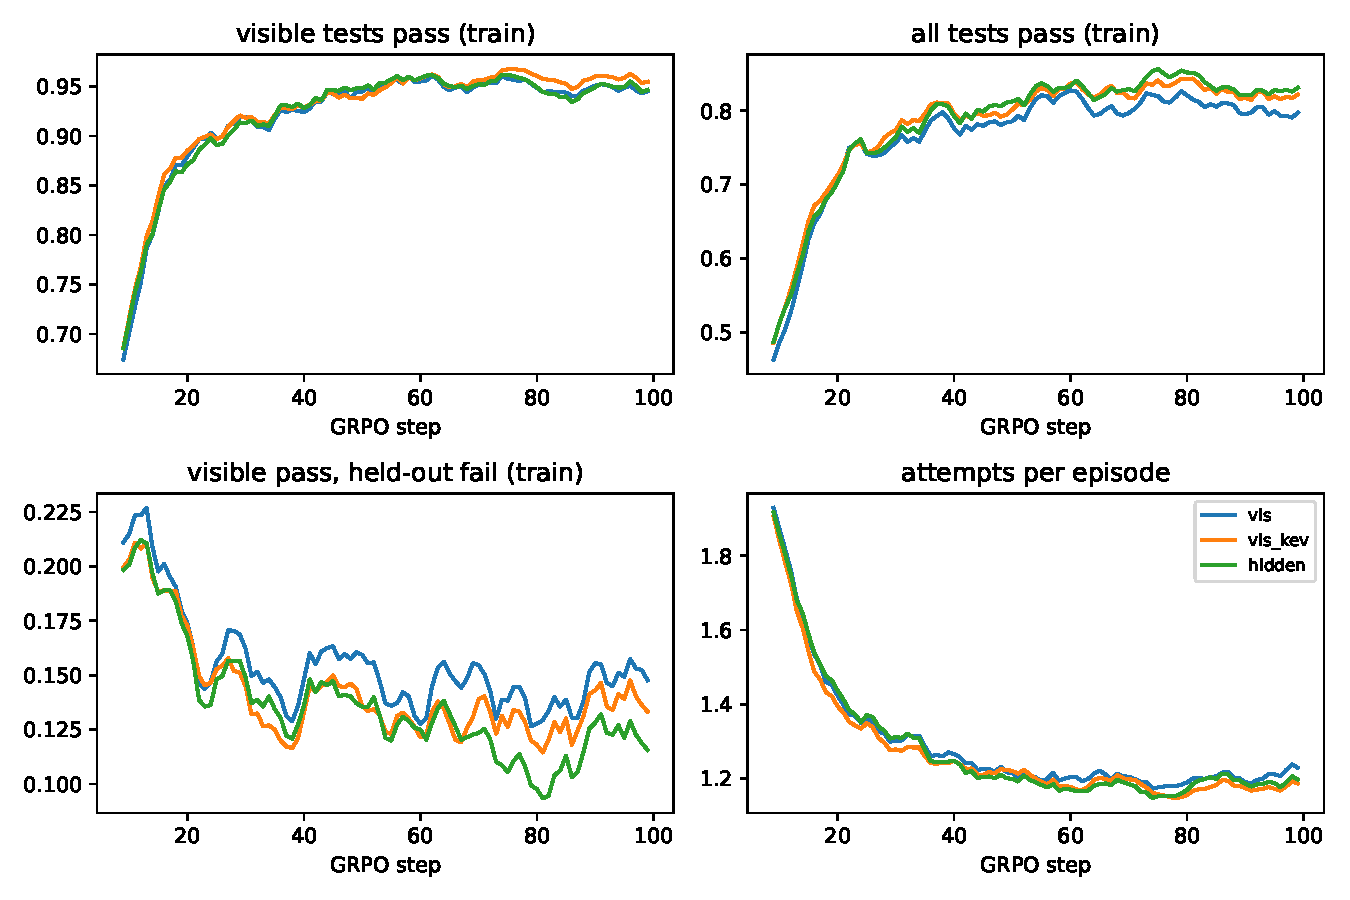
\includegraphics[width=\linewidth]{../../experiments/part3a_code/results/training_curves.pdf}
\caption{Training curves (seed mean, 10-step moving average): visible tests pass, every test passes, visible tests pass
but a held-out test fails, and attempts per episode, over the training episodes.}
\label{fig:code-curves}
\end{figure}

\paragraph{Evaluation noise.} Every run evaluates the same base model at step 0. Across the \NUM{cgszruns_kod_allpass}
runs, all-pass on KodCode validation ranges from \NUM{cgszmin_kod_allpass}\% to \NUM{cgszmax_kod_allpass}\% (standard
deviation \NUM{cgszsd_kod_allpass} points), on MBPP+ from \NUM{cgszmin_mbpp_allpass}\% to \NUM{cgszmax_mbpp_allpass}\% and
on HumanEval+ from \NUM{cgszmin_he_allpass}\% to \NUM{cgszmax_he_allpass}\%. Greedy decoding on vLLM is not bitwise
reproducible across server states. The spread between seeds of the same reward is larger: up to
\NUM{cgallsd_viskev_mbpp} points of all-pass (standard deviation, \texttt{vis\_kev} on MBPP+).
